% Preamble
% =============================================================================

% Class of the document.
\documentclass[12pt,a4paper]{article}
% article : short article.
% report  : mid-length report.
% book    : book or thesis redaction.

% Paragraph skip length (default to 0).
\setlength{\parskip}{1ex}

% Packages
% =============================================================================

% Encoding
% -----------------------------------------------------------------------------

% Babel.
\usepackage[french]{babel}
% FontEnc.
\usepackage[T1]{fontenc}
% InputEnc.
\usepackage[utf8]{inputenc}

% Define \escapeus command to escape underscores.
\makeatletter
\DeclareRobustCommand*{\escapeus}[1]{
    \begingroup\@activeus\scantokens{#1\endinput}\endgroup}
\begingroup\lccode`\~=`\_\relax
    \lowercase{\endgroup\def\@activeus{\catcode`\_=\active \let~\_}}
\makeatother

% Text
% -----------------------------------------------------------------------------

% Acronym.
\usepackage{acronym}
% CsQuote.
\usepackage[style=french,french=guillemets]{csquotes}
% Enumerate.
\usepackage{enumerate}
% HyperRef.
\usepackage[hyperfootnotes=false,hidelinks]{hyperref}
% URL.
\usepackage{url}

% Algorithms
% -----------------------------------------------------------------------------

% Algorithm2E.
\usepackage[french,onelanguage,linesnumbered,ruled,vlined,commentsnumbered]{algorithm2e}

% Source code
% -----------------------------------------------------------------------------

% Listings.
\usepackage{listings}
% Minted.
\usepackage{minted}
% Caption.
\usepackage{caption}
\newenvironment{code}{\captionsetup{type=listing}}{}

% Files
% -----------------------------------------------------------------------------

% FancyVRB.
\usepackage{fancyvrb}
% Redefine \VerbatimInput.
\RecustomVerbatimCommand{\VerbatimInput}{VerbatimInput}
{
    fontsize=\footnotesize,
    frame=lines,         % Top and bottom rule only.
    framesep=1.5em,      % Separation between frame and text.
    rulecolor=\color{red!50!green!50!blue!50!},
    labelposition=topline,
    commandchars=\|\(\), % Escape character and argument delimiters for commands within the verbatim.
    commentchar=*        % Comment character.
}

% Figures
% -----------------------------------------------------------------------------

% GraphicX.
\usepackage{graphicx}
% SVG.
\usepackage{svg}
% WrapFig.
\usepackage{wrapfig}

% Charts
% -----------------------------------------------------------------------------

% PGFPLots
\usepackage{pgfplots}
\pgfplotsset{compat=1.16}
\usepgfplotslibrary{units}
% Define style for charts.
\pgfplotsset{custom plot/.style={
        width            = 14cm,
        height           = 9cm,
        axis lines       = left,
        grid             = major,
        grid style       = {dashed},
        legend pos       = north west,
        ylabel           = Temps d'exécution,
        y unit           = \si{\second},
        enlarge y limits = upper,
        xlabel           = Optimisation,
        x unit           = \text{Valeur du define dans kernel.c},
    }
}
\pgfplotsset{custom line/.style={
        color = red,
        mark options = {
            fill = black,
        }
    }
}

% Mathematics
% -----------------------------------------------------------------------------

% AmsFonts.
\usepackage{amsfonts}
% AmsMath.
\usepackage{amsmath}
% AmsText.
\usepackage{amstext}
% AmsThm.
\usepackage{amsthm}
\newtheorem{prr}{Propriété}
\newtheorem{pro}{Proposition}
\newtheorem{thm}{Théorème}
\newtheorem{lem}{Lemme}
% NumPrint.
\usepackage{numprint}

% Physics
% -----------------------------------------------------------------------------

% Physics.
\usepackage{physics}

% Presentation
% -----------------------------------------------------------------------------

% XColor.
\usepackage{xcolor}

% References
% -----------------------------------------------------------------------------

% CleveRef.
\usepackage{cleveref}

% Structure.
% -----------------------------------------------------------------------------

% Geometry.
\usepackage{geometry}
% PDFLScape.
\usepackage{pdflscape}
% MultiCol.
\usepackage{multicol}
% TitleSec.
\usepackage{titlesec}
\newcommand{\sectionbreak}{\clearpage} % Use a page break before new sections.
% VMargin.
\usepackage{vmargin}
% FootMisc.
\usepackage[bottom]{footmisc}

% Symbols
% -----------------------------------------------------------------------------

% SIUnitX.
\usepackage{siunitx}

% Table
% -----------------------------------------------------------------------------

% Array.
\usepackage{array}
% BookTabs.
\usepackage{booktabs}
% CSVSimple.
\usepackage{csvsimple}

% Document
% =============================================================================

\begin{document}

\title{Analyse de performance et optimisation de code}
\author{AYOUB Pierre -- BONNAFOUS Camille -- FLAMANT Océane}

\maketitle

\begin{figure}[b]
    \centering
    
\includegraphics[scale=0.3]{figures/isty.jpg}
\end{figure}

\newpage
\begin{abstract}

La simulation numérique est un procédé informatique visant à modéliser un
phénomène par ordinateur, s'agissant le plus souvent d'un phénomène
physique. Cette modélisation prend forme par des systèmes d'équations
décrivant l'état du système physique représenté à chaque instant. De
nombreux domaines scientifiques convergent vers la simulation
informatique, tel que certaines branches de la physique, de l'analyse
et de l'optimisation mathématique, ou encore le calcul haute
performance en informatique. Enfin, la simulation trouve naturellement
de nombreuses applications concernant des sujets variés, tel que la
simulation du climat et des évènements météorologiques, la simulation
d'essais nucléaires, de l'effet d'un médicament sur un corps, ou encore
des astres et de l'univers. Ce rapport s'articulera donc autour de l'analyse et
de l'optimisation d'un code de calcul, cœur des simulations numériques
présentés ci-dessus.

\end{abstract}

\tableofcontents

\section{Introduction}

Le projet que nous vous présentons aujourd'hui consiste à analyser puis, grâce à
nos mesures, optimiser un code de calcul, appelé kernel. Les mesures doivent
s'effectuer à l'aide de l'instruction \textit{x86} \textit{RDTSC}, et des deux
outils d'analyse de performance suivant : \textit{MAQAO} et \textit{LIKWID}.
\textit{RDTSC} nous permet de mesurer le nombre de cycles entre deux instants,
\textit{MAQAO} rends possible l'exécution d'analyses statiques (\textit{CQA}) et
dynamiques (\textit{LPROF}) d'un binaire, présentées par un rapport haut niveau
à l'aide de \textit{ONE-VIEW}, enfin \textit{LIKWID} permet d'obtenir un grand
nombre de métriques très précises concernant, notamment, l'usage de la mémoire.

Afin d'étudier les différents niveaux de la hiérarchie mémoire, chaque membre du
groupe analysera un niveau qu'il se verra assigné. Ci-dessous la liste des
assignations :
\begin{description}
    \item[Pierre] Cache L1 : 
        \begin{itemize}
            \item Intel Core i7-6600U @ 2.8 GHz, Skylake $6^{\text{ème}}$ génération, 14nm, 2 cœurs 4 threads (Hyper-Threading)
            \item 32 KiB L1i, 32 KiB L1d (par coeur)
            \item 256 KiB L2 (par coeur)
            \item 4096 KiB L3 (partagé)
        \end{itemize}
    \item[Océane] Cache L2 : 
        \begin{figure}[!h]
		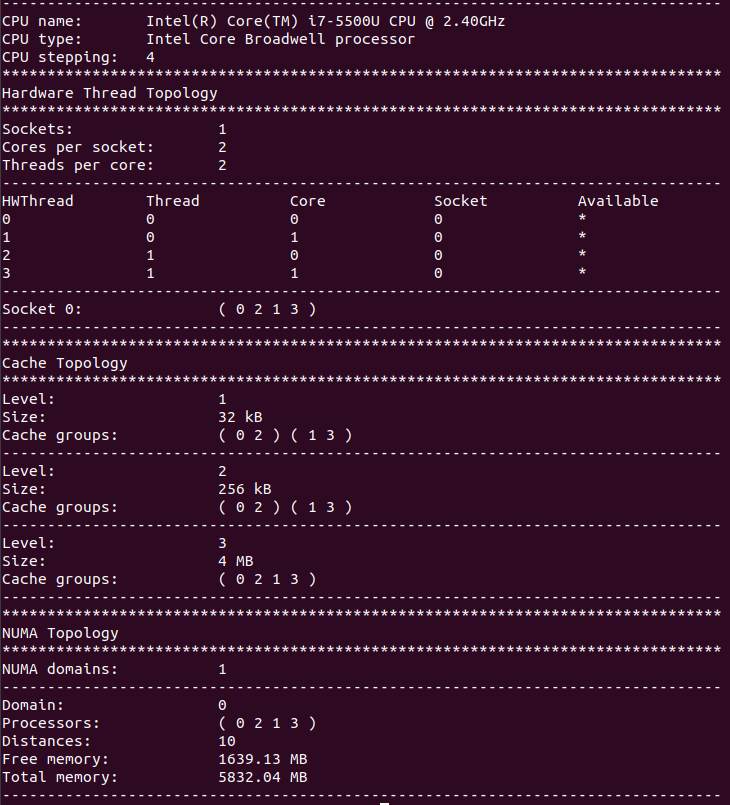
\includegraphics[scale=0.42]{figures/L2/L2topo.png}
		\caption{ }
        \end{figure}
    \item[Camille] RAM : 
        \begin{itemize}
            \item Voir le fichier \enquote{.odt} annexe envoyé par Camille.
        \end{itemize}
\end{description} 

Le déroulement du projet s'est effectué en plusieurs étapes distinctes :
\begin{description}
    \item[Analyse du code] Cette phase consiste à analyser le programme d'un
        point de vue d'architecture informatique. Il convient d'étudier les
        choix mis en œuvres afin d'implémenter le ou les calculs nécessaires.
    \item[Protocole expérimental] Une fois l'analyse effectuée, nous
        pouvons en déduire le moyen le plus adapté afin de mesurer les
        performances de notre implémentation. Nous allons donc mettre en
        avant les critères théoriques à atteindre dans nos mesures, puis
        nous exposerons la manière dont nous avons mis ceci en pratique.
    \item[Optimisations et mesures] Grâce au protocole mis en place, nous
        pouvons quantifier la performance du programme. De ce fait, nous serons
        en mesure d'expérimenter différentes techniques d'optimisation sur le
        programme et d'en calculer l'accélération.
\end{description}

\section{Analyse du code}

Présentons notre kernel par son prototype, que nous observons sur le
Listing~\ref{lst.baseline.noopt.prot} Nous voyons qu’il y a 3 variables qui sont manipulées :
\begin{itemize}
    \item $n$ correspond à la taille de nos tableaux.
    \item $a$ est un tableau de \textit{float} à deux dimensions dont la taille
        en fonction de $n$ : $4n^2$ Bytes.
    \item $b$ est un tableau de \textit{double} à une dimension dont la taille
        en fonction de $n$ : $8n$ Bytes.
\end{itemize}

\begin{listing}[h]
    \begin{minted}[linenos,numbersep=5pt,frame=lines,framesep=2mm]{C}
void baseline(unsigned n, float a[n][n], double b[n])
    \end{minted}
    \caption{Prototype du kernel non-optimisé}
    \label{lst.baseline.noopt.prot}
\end{listing}

Nous sommes face à un code de calcul très simple en apparence, illustré dans le
Listing~\ref{lst.baseline.noopt} : deux boucles imbriquées, un branchement, un
calcul mêlant multiplication et exponentiel. Mais plusieurs éléments remarquables qui
risquent de poser problème au niveau de la rapidité d'exécution apparaissent
alors : les boucles impliquent qu'il faut prêter attention au sens de parcours
des tableaux, le branchement nous laisse penser qu'il faudrait essayer de le
supprimer, enfin l'exponentiel et la multiplication sont des opérations lourdes.

\begin{listing}[h]
    \begin{minted}[linenos,numbersep=5pt,frame=lines,framesep=2mm]{C}
for (j = 0; j < n; j++) {
    for (i = 0; i < n; i++) {
        if (j == 0)
            b[i] = 1.0;
        b[i] *= exp(a[i][j]);
    }
}
    \end{minted}
    \caption{Kernel non-optimisé}
    \label{lst.baseline.noopt}
\end{listing}

\section{Protocole expérimental}

La mise en place d'un protocole expérimental de mesure est une étape nécessaire
et cruciale dans tout processus d'optimisation de code. D'une part, le but de ce
protocole est de mettre en lumière les points chauds du programme, c'est-à-dire
les parties du code qui ralentissent considérablement l'exécution des calculs :
ces points chauds seront les cibles de nos optimisations. D'autre part, après
chaque tentative d'optimisation, le protocole doit nous permettre de mesurer
l'impact de cette dernière, qu'il soit positif ou négatif, et enfin de le
quantifier.

\subsection{Driver}

Le code de notre environnement de mesure est séparé en deux parties : le \textit{driver}
et le \textit{kernel}. Le kernel contient la fonction de calcul à proprement
dite, sur laquelle nos optimisations se porteront. Le driver est le code qui
nous permet d'effectuer nos mesures. Le paragraphe suivant sera consacré à une
rapide explication de son fonctionnement, le code étant accessible dans le fichier
\enquote{\textit{driver.c}}.

Les premières lignes du driver servent à récupérer les options de mesures
passées en argument à l'application. Vint ensuite une boucle qui englobe toute
l'expérience de mesure, elle correspond à l’exécution des méta-répétitions. Une
méta-répétition est une répétition qui comprend l'expérience dans sa globalité.
L'utilité d'avoir plusieurs méta-répétitions vient du fait que plusieurs mesures
sont nécessaire pour être représentatives, car une mesure isolée pourrait être
biaisée. On prend la mesure médiane issues des différentes méta-répétitions. Les
premières lignes de la boucle des méta-répétitions correspondent à l'allocation
et l'initialisation des tableaux utilisés par le kernel. Il faut faire attention
à bien utiliser la mémoire lors de l'initialisation, sinon \textit{Linux}
pourrait ne pas vraiment allouer le tableau en mémoire (initialisation
paresseuse). Ensuite, nous entrons dans une petite boucle qui effectue le
warmup, c'est-à-dire la \enquote{mise en chauffe} (terme vague mais expliquant
le nom) du processeur. Derrière cette appellation grossière se cache un
remplissage de la mémoire cache avec nos tableaux, puisque l'on effectue
plusieurs fois la fonction de calcul \enquote{dans le vide}, sans effectuer de
mesure. Cette phase de warmup permet de passer le régime transitoire, ou le
temps de calcul s'améliore à chaque itération, pour arriver dans le régime
permanent, ou le temps de calcul est stable. Une fois le warmup terminé, on
passe à la mesure proprement dite, effectué par l'instruction \textit{RDTSC}. Le
choix s'est porté sur cette instruction pour son efficacité : en effet, elle
appelle directement une instruction assembleur x86 correspondante, et son
imprécision n'est que de quelques dizaines de cycles seulement. Entre nos deux
instructions \textit{RDTSC} (start/stop) se trouve une boucle de répétition
d'appel du kernel. Cette boucle de répétition est nécessaire afin d'avoir une
mesure précise : il se trouve que si on effectuait un seul appel au kernel, il
se pourrait que les instructions de mesure (\textit{RDTSC}) et de contrôle
prennent autant ou plus de temps que le code de calcul, ce qui biaiserait
complètement les résultats. Il faut donc faire plusieurs répétitions afin
d'avoir un temps de calcul conséquent par rapport au reste des instructions.

\subsection{Théorie}

Lors de nos expériences, de nombreux paramètres peuvent être sujets à des
variations aléatoires ou à des erreurs de mesure, ainsi un résultat peut être
biaisé. Afin d'éviter cela, il est impératif d'utiliser une valeur
représentative de nos différentes mesures : une valeur moyenne ou une valeur
médiane. La valeur médiane semble être un meilleur candidat contrairement à la
moyenne, car cette dernière peut-être fortement modifié par une valeur extrême
qui n'as pas lieu d'être. C'est donc la valeur médiane que nous prendrons des
résultats de nos mesures successives issues des méta-répétitions.

Pour que chaque membre de l'équipe puisse travailler sur son niveau de mémoire
cache, il nous faut trouver la taille des données d'entrée à utiliser. Selon le
prototype présenté dans le Listing~\ref{lst.baseline.noopt.prot}, la taille
totale de nos données d'entrées est de $4n^2 + 8n$, avec $n$ la taille entrée
en paramètre du programme.

\subsubsection{Cache L1}

Ci-dessous les paramètres des mesures :
\begin{enumerate}[(1)]
    \item Taille pour tenir dans L1 : $n = 88$.
        En effet, $(n^2 * 4) + (n * 8) = 31680 B$, sachant que la taille du
        cache est de $32 kiB = 2^{15} = 32768 B$, et que si l'on prend $n =
        90$, on obtient $33120 B$, on a bien : $n = 88 < L1 < n = 90$ avec une
        bonne marge de sécurité.
    \item Nombre de répétitions du warm-up : 1000. Ce nombre est suffisant pour
        avoir ensuite des mesures stables dans tous nos tests car les caches
        sont remplis avec nos tableaux, choisi par observation. Il permet donc
        de passer le régime transitoire.
    \item Nombre de répétitions des mesures : on choisit un nombre qui nous
        permet d'avoir un temps minimum représentatif par méta-répétition. Ce
        nombre varie en fonction de la taille de notre tableau. Avoir plus ou
        moins 1 seconde de mesures permet d'avoir une faible marge d'erreur de
        mesures des cycles avec un \textit{RDTSC}. Par exemple, pour une taille
        de 89, on peut choisir 10000.
\end{enumerate}

\subsubsection{Cache L2}

Pour que les deux tableaux entrent entièrement dans le cache L2, il faut 
que la formule respecte les contraintes suivantes : 
\begin{itemize}
    \item La taille totale doit être plus grande que la taille du cache 
    L1 (1). Pour plus sécurité il a été décidé que la taille totale devait 
    être au moins trois fois plus grande que celle du L1.
    \item L2 partage sa mémoire pour stocker à la fois les instructions, 
    les données et ce qui tourne en background, on ne peut donc en utiliser 
    approximativement que 90\% (2). 
\end{itemize}

Ces deux contraintes peuvent être transformées sous forme d'inéquation :
\begin{itemize}
    \item (1) : $3*TL1 < 4n*n + 8n$,
    \item (2) : $4n*n + 8n \le 0,9*\text{TL2}$
\end{itemize}
Après la résolution de ces équations on obtient $n=156$ comme minimum et $n=242$
comme maximum.

\subsubsection{RAM}

Voir le fichier \enquote{.odt} annexe envoyé par Camille.

\subsubsection{Analyse de sensibilité}

Une fois que l'on connaît la taille des données a fournir en entrée, 
il faut effectuer une analyse de sensibilité pour les autres paramètres. 
\begin{description}
    \item[Nombre de méta-répétition des mesures] Il nous est donné à 31. C'est
        le nombre donné dans la consigne, qui est suffisant pour avoir un nombre
        de mesure significatives.
    \item[Le nombre de warmup] Il doit se situer entre 1 et 1000. Pour le
        déterminer, il doit être le seul paramètre que l'ont fait varier. On
        fait plusieurs exécutions et, avec les valeurs obtenues, on fait une
        courbe pour voir à partir de quelle valeur cela devient stable. Il faut
        aussi vérifier que
        $\frac{\text{médiane}-\text{minimum}}{\text{minimum}}$ est inférieur à
        5\%. 
    \item[Le nombre de répétitions] On le trouve de la même manière que le
        nombre de warmup.
\end{description}

\subsection{Pratique}

Lors de nos premières tentatives pour trouver les paramètres, nous avons remarqué
que ce qui prenait le plus de temps dans notre noyau de calcul était
l'exponentiel. Afin de pouvoir vérifier si nos paramètres sont corrects, nous
avons donc modifié le fichier \textit{kernel.c} pour que ce soit le temps de
récupération des données qui soit le plus grand. Cette version n'est utilisé que
pour tester la véracité des paramètres trouvés dans la section précédente, et
non pas pour évaluer les performances des optimisations ou des compilateurs.

\subsubsection{Cache L1}

On peut observer une nette différence de performance entre un $n = 88$ et un $n
= 90$, qui se traduit par le fait de tenir ou de ne pas tenir en cache
\textit{L1}. On assigne le programme de calcul au cœur n°2 de la machine avec
\textit{taskset}, sur son numéro de thread physique, dans le but de limiter les
changements de contexte et de flush de la mémoire cache. Les tests sont
effectués en rescue/failsafe mode, sans interface graphique, permettant d'avoir
un minimum de tâches tournant en arrière-plan. De plus, le gouverneur du
processeur est sélectionné sur le mode performance et la fréquence est fixé. Toutes
les mesures effectuées dans le cache L1 sont automatisées par un script
(\textit{report/L1/P\{1,2\}/bench.sh}). Ce script permet d'aisément exécuter
l'ensemble des tests dans un environnement idéal, ainsi que d'assurer la
reproductibilité du protocole expérimental, critère important d'une méthode
scientifique. Les compilateurs utilisés sont \textit{GCC v8.3.0}, \textit{Clang
v7.0.1}, \textit{ICC v19.0.2.187}, tournants sur un \textit{Debian v10 Buster
(testing)} composé du noyau \textit{Linux v4.19.0 x86\_64}.

\subsubsection{Cache L2}
Avant de pouvoir executer et mesurer quelque chose il faut s'assurer que 
la machine n'utilise pas son temps de calcul ou d'accès à la mémoire pour 
autre chose que notre programme. Pour cela il faut passer en mode root qui 
n'utilise pas d'interphase graphique et n'est pas connecté au réseau. On 
connecte la machine au secteur pour qu'elle ne se mette pas en mode economie
d'energie. Il faut ensuite ffixer la fréquence à l'aide de \textit{cpupower 
frequency-set} et enfin lorsque l'on compile le programme il faut aussi fixer
le coeur afin d'éviter que le programme s'execute sur plusieurs et qu'il 
faille transferer des données entre les différents coeurs ce qui ferrait 
perdre du temps. Pour fixer le coeur on utilise taskset.

Pour vérifier le calcul théorique de la taille des données j'ai utilisé
likwid-perftcr afin de voir si les données transitaient bien par le cache L2.
Après avoir compilé avec gcc uniquement j'ai exécuté l'exécutable avec likwid et
voici les résultats obtenus :

\begin{table}[!h]
    \centering
    \begin{tabular}{|c|c|}
        \hline
        n & Data Volume (GByte) \\
        \hline
        100 & 4,24 \\
        \hline
        150 & 14,06 \\
        \hline
        220 & 37,9 \\
        \hline
        235 & 34,4 \\
        \hline
    \end{tabular}
\end{table}

On observe que ces résultats sont en corrélation avec les résultats théoriques :
en dessous de 156 pratiquement aucune donnée ne passe par le cache L2, et 
quand on se rapproche de 242 une partie des données ne semble plus passer 
dans L2. Je suppose donc que ces données vont directement dans le cache L3.
Au vu de ces informations, j'ai choisi de prendre 220 comme taille de 
données.

Voici ci-contre le graphique obtenu pour trouver le bon nombre de warmup. On
peut observer que le nombre de cycles semble se stabiliser au alentour de 100
warmup. Pour plus de sécurité j'ai choisi 150 pour le nombre de warmup.

\begin{figure}[!h]
    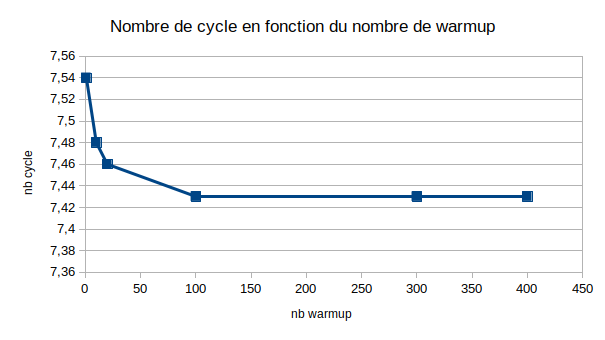
\includegraphics[scale=0.8]{figures/L2/L2warmup.png}
    \caption{Sans l'exponentiel}
\end{figure}

J'ai ensuite vérifié avec le calcul de l'exponetiel et on obtient bien le 
même résultat. 

\begin{figure}[!h]
    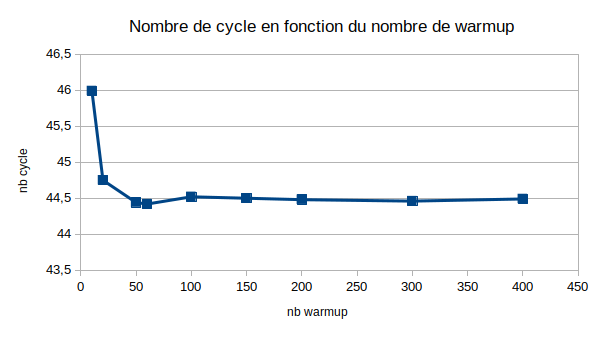
\includegraphics[scale=0.8]{figures/L2/L2warmup2.png}
    \caption{Avec l'exponentiel}
\end{figure}

Pour trouver le bon nombre de répétitions j'ai uniquement fait les tests avec
l'exponentiel. Comme vous pouvez le voir, on peut remarquer que l'ensemble est
stable, les variations sont minimes. J'ai choisit comme nombre de répétitions
1200.
\begin{figure}[!h]
    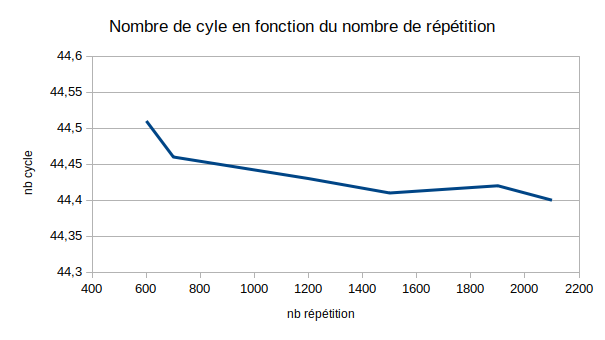
\includegraphics[scale=0.8]{figures/L2/L2repet.png}
    \caption{ }
\end{figure}

\subsubsection{RAM}

Voir le fichier \enquote{.odt} annexe envoyé par Camille.

\section{Optimisations et mesures}

Dans cette section, nous présentons les résultats des mesures des différentes
tentatives d'optimisation du code. La phase 1 correspond, pour résumer, à
identifier les points chauds et tester différentes configurations de compilation.
La phase 2 correspond, notamment, à une optimisation active du code en y apportant
des modifications.

\subsection{Phase 1}

\subsubsection{Cache L1}

Pour cette première phase de test sur un jeu de donnée dans le niveau de cache
L1, nous avons testé 3 compilateurs (\enquote{gcc}, \enquote{icc},
\enquote{clang}) avec différents jeux de flags de compilation. Nous précisons que
l'intégralité de nos résultats sont disponibles sous formes brut dans les
fichiers/répertoires suivants : \enquote{compil.txt},
\enquote{likwid\_\{ref,opt\}}, \enquote{maqao\_\{ref,opt\}}.

En plus des flags qui sont donnés dans la consigne, nous avons également testé
le flag \enquote{-Ofast} qui permet d'activer des optimisations mathématiques qui
ne respecte pas les standards en vigueur. Un programme qui ne requiert pas une
stabilité numérique très précise obtiendra des gains considérable avec cette
option, cependant, cela peut être dangereux de l'activer sans possibilité de
vérifier les résultats des calculs du kernel. Nous avons ici pris le pari de
l'activer.

Nous avons aussi testés d'autres options ciblées :
fonctions inline, optimisations sur les boucles, sur les fonctions
mathématiques ou encore sur les branchements. La liste ci-dessous présente
les flags qui n'auront pas apporté de gain, ou pire, auront provoqué une accélération
négative par rapport à \enquote{-Ofast -march=native} :
\enquote{-faggressive-loop-optimizations}, \enquote{-fbranch-probabilities},
\enquote{-fdelayed-branch}, \enquote{-fexpensive-optimizations},
\enquote{-finline-functions}, \enquote{-floop-block},
\enquote{-floop-interchange}, \enquote{-floop-unroll-and-jam},
\enquote{-funsafe-math-optimizations}. Cependant, le flag
\enquote{-funroll-all-loops}, permettant de forcer l'unrolling des boucles, nous
aura octroyé un léger gain systématique.

Dans la Table~\ref{tab.compil} est présenté la liste des résultats sur les flags
obligatoires et les flags apportant un gain (les flags inutiles ou ralentissant
ne sont pas inclus pour des soucis de visibilité). Nous pouvons ainsi voir que
c'est \enquote{gcc}, couplé à certaines options, qui est le plus rapide face à
\enquote{clang} et \enquote{icc}. Nous notons tout de même l'efficacité
redoutable de la génération de code spécialement pour l'architecture hôte
(\enquote{-march=native}), permettant d'utiliser les instructions x86 les plus
récentes, et des optimisations mathématiques agressives (\enquote{-Ofast}).

\begin{table}[h]
    \centering
    \begin{tabular}{l|l|l}
        \bfseries Compiler & \bfseries Flags & \bfseries Time (s)
        \csvreader{./L1/P1/compil.txt}{}
        {\\\hline\csvcoli&\csvcolii&\csvcoliii}
    \end{tabular}
    \caption{Benchmarks des compilateurs et flags}
    \label{tab.compil}
\end{table}

Nous avons ensuite utiliser les outils \textit{MAQAO} et \textit{LIKWID} pour
expliquer les différences de performances entre deux versions du code. Après nos
tests avec notre script permettant de détecter les flags permettant d'avoir le
meilleur speed-up, nous allons étudier les différences de performances entre la
version de référence \enquote{gcc -O2} et la version la plus rapide,
\enquote{gcc -Ofast -march=native -funroll-all-loops}.

Procédons tout d'abord à une analyse rapide avec \textit{LIKWID}, les résultats
étant présentés dans la Figure~\ref{fig.likwid_noopt}. Nous pouvons expliquer
la différence de performance par les métriques suivantes concernant la mémoire :
on observe que la version optimisé à fait un nombre significativement moins
important que la version de référence d'éviction de données du cache L1 (2.051.211
vs. 16.140.154), ainsi qu'un ratio de miss bien plus faible dans le cache L2
(0.0001 vs. 0.0259).

\begin{figure}[h]
    \centering
    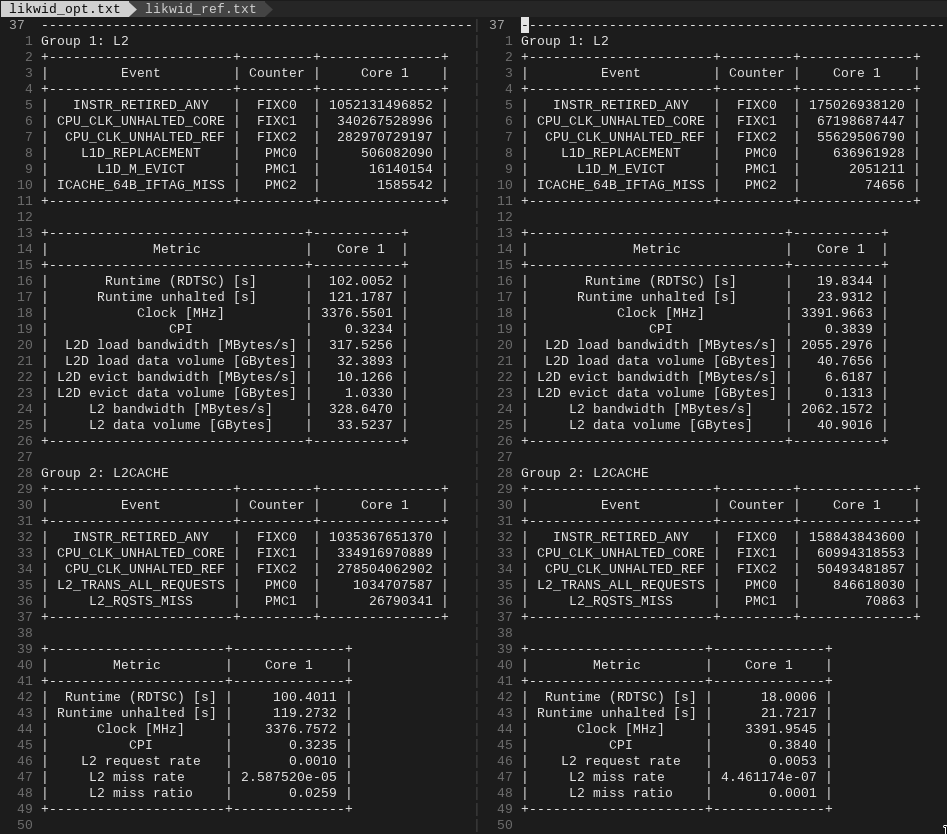
\includegraphics[scale=0.45]{./figures/L1/likwid_noopt.png}
    \caption{A gauche, la version de référence. A droite, la version avec les
    flags d'optimisation.}
    \label{fig.likwid_noopt}
\end{figure}

Enfin, passons à l'étude avec MAQAO. Sur le page \enquote{Global} présenté par
la Figure~\ref{fig.maqao_noopt_global}, nous pouvons déjà avoir une très bonne
idée des différences entre les deux binaires, justifiant d'une telle
accélération ($\text{acc} = \frac{212}{41} = 5.2$). Premièrement, nous observons
que sur le binaire optimisé, nous passons deux fois plus de temps dans la boucle
que dans la version de référence : cela signifie que les fonctions
mathématiques (multiplication, mais surtout l'exponentiel) ont été
considérablement optimisées. Ensuite, nous voyons que la version de référence
présente deux chemins (Flow Complexity) dans la boucle, tandis que la version
optimisée ne présente qu'un chemin d'exécution possible. Nous notons aussi que
l'efficacité d'accès aux données (Array Access Efficiency) a été augmenté de
20\% dans la version optimisée, sûrement par modifications des boucles
imbriquées. Enfin, nous pouvons imaginer une tentative de vectorisation de la
part du compilateur pour la version optimisée.

\begin{figure}[p]
    \centering
    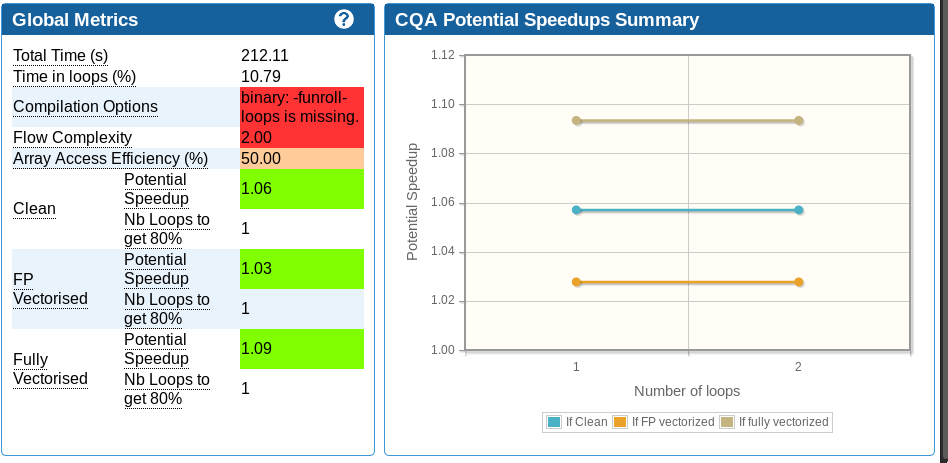
\includegraphics[scale=0.5]{./figures/L1/maqao_noopt_ref_global.png}
    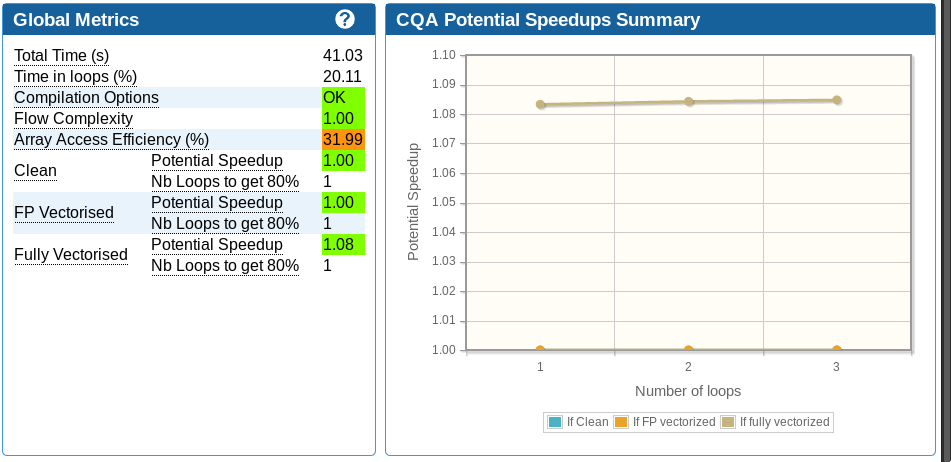
\includegraphics[scale=0.5]{./figures/L1/maqao_noopt_opt_global.png}
    \caption{Au-dessus, la version de référence. En dessous, la version avec les
    flags d'optimisation.}
    \label{fig.maqao_noopt_global}
\end{figure}

Pour finir avec l'analyse de \textit{MAQAO}, sur la
Figure~\ref{fig.maqao_noopt_func}, nous pouvons observer ce qu'à concrètement
fait le compilateur. La fonction exponentielle, qui prenait 14\% du temps, à été
remplacé par une version optimisée \enquote{fini}, ne prenant plus que 1.46\% du
temps. Nous pouvons voir que le linkage de la bibliothèque mathématique
(\textit{libm}) a été remplacé par sa version vectorisée (\textit{libmvec}).
Enfin, nous observons que notre unique boucle à bien été déroulée car nous
trouvons l'ajout d'une \textit{tail loop}.

\begin{figure}[h]
    \centering
    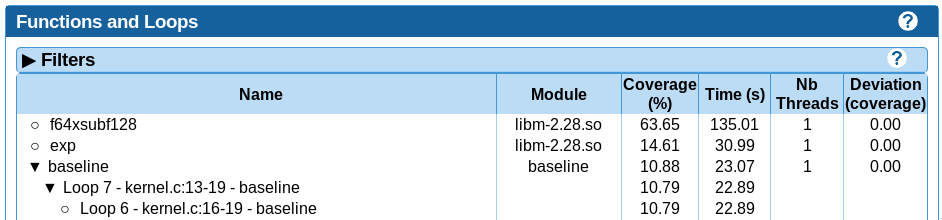
\includegraphics[scale=0.5]{./figures/L1/maqao_noopt_ref_func.png}
    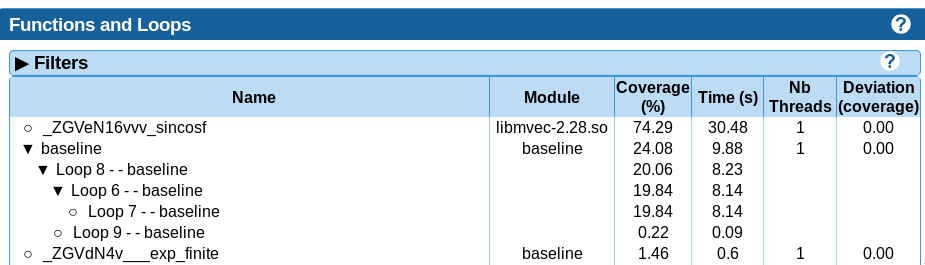
\includegraphics[scale=0.5]{./figures/L1/maqao_noopt_opt_func.png}
    \caption{Au-dessus, la version de référence. En dessous, la version avec les
    flags d'optimisation.}
    \label{fig.maqao_noopt_func}
\end{figure}

\subsubsection{Cache L2}

\begin{table}[h]
    \centering
    \begin{tabular}{|c|c|c|}
        \hline
        Numéro & Commande & Résultat (médiane)\\
        \hline
        1 & gcc -O2 & 39,93 \\
        \hline
        2 & gcc -O3 & 37,62 \\
        \hline
        3 & gcc -O3 -march=native & 37,79 \\
        \hline
        4 & icc -O2 & 17,79 \\
        \hline
        5 & icc -O3 & 17,77 \\
        \hline
        6 & icc -O3 -xHost & 17,74 \\
        \hline
    \end{tabular}
\end{table}

On remarque avec ces résultats que icc rend l'exécution plus rapide que 
gcc, néanmoins, les différentes options d'optimisation n’ont pas un impact
considérable contrairement à gcc qui entre O2 et O3 gagne quelques secondes.

À l'aide de LIKWID, on peut observer que le volume de data est différent 
entre l’exécution avec icc et gcc, il est d'environ 37 GBytes avec gcc et
7 GBytes avec icc. Le miss rate est équivalent entre les deux compilateur.

\subsubsection{RAM}

Voir le fichier \enquote{.odt} annexe envoyé par Camille.

\newpage
\subsection{Phase 2}

La phase 2 constituait en un exercice d'application d'optimisation, en ceci que
nous avons recommencé à utiliser notre version du programme par défaut
(\textit{gcc -O2}) pour appliquer des optimisations manuelles au niveau du code
source. Dans les sections suivantes, nous allons vous présenter, pour chaque
niveau de mémoire étudiée, les optimisations ayant été faites. Pour des raisons de
visibilité, le code ne sera pas inclus dans ce rapport : toutes les optimisations
vont visibles dans le fichier \enquote{kernel.c}.

\subsubsection{Cache L1}

La Figure~\ref{fig.compare-optims} nous permet de comparer les différents temps
d'exécution des différentes optimisations. Nous observons d'emblée qu'une
optimisation nous fait perdre des performances (OPT-OMP), tandis que les autres
optimisations apportent des améliorations minimes. Enfin, on observe qu'à
l'optimisation de la fonction exponentielle (OPT-EXP), les gains de performances
sont très nets. Nous allons détailler les optimisations dans les prochains
paragraphes. On remarquera qu'il n'y a pas d'analyse des rapports de LIKWID dans
les sections suivantes : en effet, une fois en L1, la mémoire n'est pas un
facteur limitant des performances de notre code comparé aux calculs. Par
conséquent, LIKWID ne nous a pas été utile à ce niveau.
\begin{figure}[h]
    \begin{center}
        \begin{tikzpicture}
            \begin{axis} [
                    custom plot,
                    title = Mesures effectuées à l'aide de RDTSC,
                    xtick = data,
                    symbolic x coords = {
                        OPT-OMP, OPT-LOOP-STRIDE-1, NOOPT, OPT-RESTRICT,
                        OPT-IF-HOISTING, OPT-LOOP-UNROLLING, OPT-EXP1, OPT-EXP2,
                        OPT-BEST-L1, OPT-BEST-L1-2,
                    },
                    xticklabel style = {
                        rotate=50,
                    },
                ]
                \addplot+[custom line] table [
                    x       = version,
                    y       = time,
                    col sep = comma,
                ] {L1/P2/rdtsc.txt};
            \end{axis}
        \end{tikzpicture}
        \caption{Temps d'exécution en fonction de l'optimisation}
        \label{fig.compare-optims}
    \end{center}
\end{figure}

\paragraph{Accès séquentiel au tableau (OPT-LOOP-STRIDE-1)} MAQAO nous indique,
dans la Figure~\ref{fig.maqao_noopt_non-unit-stride}, que l'efficacité d'accès
aux tableaux est mauvais (50\% d'efficacité). En inversant la boucle intérieure
et extérieure, on améliore l'efficacité à 58\%, comme illustré par la
Figure~\ref{fig.maqao_noopt_unit-stride}. Si on enlève en plus le \textit{if}
(une autre optimisation), cette efficacité passe alors à 75\%. Cependant, malgré
cette meilleure efficacité, le gain de performances est négligeable : l'accès à la
mémoire n'est pas le facteur limitant de notre kernel.

\begin{figure}[h]
    \centering
    
\includegraphics[scale=0.4]{./figures/L1/maqao_noopt_non-unit-stride.png}
    \caption{Rapport de MAQAO sur NOOPT : accès non-stride 1.}
    \label{fig.maqao_noopt_non-unit-stride}
\end{figure}

\begin{figure}[h]
    \centering
    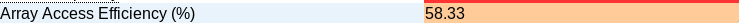
\includegraphics[scale=0.4]{./figures/L1/maqao_noopt_unit-stride.png}
    \caption{Rapport de MAQAO sur OPT\_LOOP\_STRIDE\_1 : augmentation de l'efficacité.}
    \label{fig.maqao_noopt_unit-stride}
\end{figure}

\paragraph{Suppression du \textit{if} (OPT-IF-HOISTING)} La
Figure~\ref{fig.maqao_noopt_if} nous montre que le fait d'avoir deux chemins
possible dans la boucle limite les performances, de plus MAQAO nous indique un
\textit{Flow Complexity} de 2. Une fois le \textit{if} isolé dans une boucle
appart qui se fait avant la boucle principale, nous avons un \textit{Flow
Complexity} de 1 et plus d'avertissement concernant de multiples chemins à
l'intérieur de la boucle. On observe un très léger gain au niveau des
performances, mais encore une fois, deux chemins possibles (empêchant un
pipelining optimale) n'est pas un facteur très limitant par rapport au reste.

\begin{figure}[h]
    \centering
    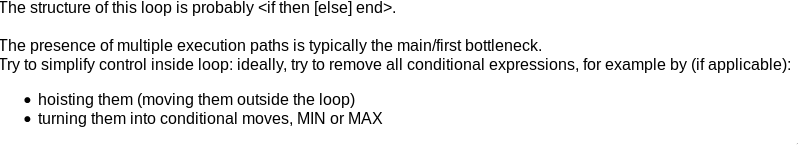
\includegraphics[scale=0.4]{./figures/L1/maqao_noopt_if.png}
    \caption{Rapport de MAQAO sur NOOPT : chemins multiples.}
    \label{fig.maqao_noopt_if}
\end{figure}

\paragraph{Déroulage de boucle (OPT-LOOP-UNROLLING)}
MAQAO nous indiquait une possibilité d'unroller notre boucle si notre nombre
d'itération est significativement plus élevée que le facteur d'unrolling, ce qui
est le cas ici (Figure~\ref{fig.maqao_noopt_unroll}). Une fois l'unrolling de la
boucle intérieure effectué avec un facteur de 2, nous observons un très léger
gain de performances puisque l'on peut commencer à effectuer la prochaine
itération avant la fin de la première. Encore une fois, le gain n'est pas
significatif.

\begin{figure}[h]
    \centering
    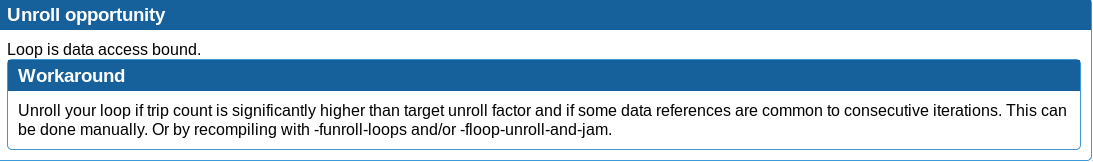
\includegraphics[scale=0.4]{./figures/L1/maqao_noopt_unroll.png}
    \caption{Rapport de MAQAO sur NOOPT : possiblité d'unrolling.}
    \label{fig.maqao_noopt_unroll}
\end{figure}

\paragraph{Pointeurs restreints (OPT-RESTRICT)}
Nous avons utilisé le mot-clé \textit{restrict} pour indiquer que les pointeurs
pointait sur des zones de mémoire distinctes et indépendantes entre elles. Cela
permet notamment au compilateur de plus facilement vectoriser le code et
ré-arranger l'ordre des instructions, puisqu'il y a moins de
\enquote{précaution} à prendre. Ici, c'est une optimisation extrêmement légère,
mais qui peut parfois révéler de bonnes surprises.

\paragraph{Utilisation de l'exponentielle sur un float (OPT-EXP-1)} La
bibliothèque standard propose plusieurs versions de l'exponentielle, dont une
pour un double (par défaut) et une pour un float. Celle pour un float est
naturellement moins précise, mais permet en revanche d'être extrêmement plus
rapide. En effet, MAQAO nous indiquait que la majorité du temps de notre kernel
était passé dans la bibliothèque de mathématiques, voir la
Figure~\ref{fig.maqao_noopt_bottleneck}. En utilisant la fonction exponentielle
sur un float, on améliore significativement les performances : on obtient un
speed-up d'environ $2.3$.

\begin{figure}[h]
    \centering
    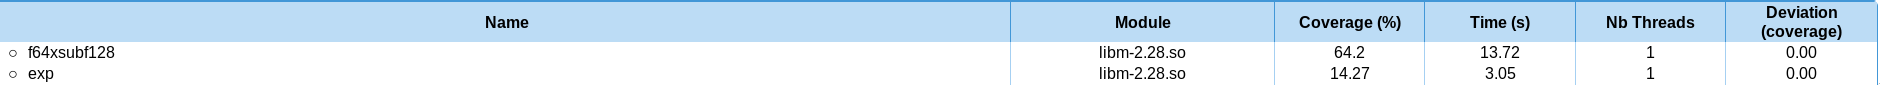
\includegraphics[scale=0.25]{./figures/L1/maqao_noopt_bottleneck.png}
    \caption{Rapport de MAQAO sur NOOPT : fonction exponentielle limitante.}
    \label{fig.maqao_noopt_bottleneck}
\end{figure}

\paragraph{Utilisation d'une fonction exponentielle custom (OPT-EXP-2)} Afin
d'améliorer la rapidité de la fonction exponentielle, nous avons décidé de
programmer notre propre version. Cette version est précise pour un $x$ faible
($< 5$), et permet d'obtenir un speed-up considérable par rapport à
l'exponentielle originale. Par rapport à l'exponentielle sur float, elle
apporte un petit gain de performances. Nous savons qu'utiliser cette
approximation n'est pas un problème puisque les valeurs de notre tableau $a$
sont comprises entre -1 et 1. L'explication de l'optimisation est la suivante.
La fonction exponentielle est définie par la série entière suivante :
\begin{equation*}
    \exp(x) = \sum^{\infty}_{k=0} \frac{x^k}{k!} = 1 + x + \frac{x^2}{2} + \frac{x^3}{6} + \frac{x^4}{24} + ...
\end{equation*}
En appliquant le développement de série entière puis la formule du binôme de
Newton, on peut exprimer la fonction exponentielle de cette manière :
\begin{equation*}
    \exp(x) = \lim_{n \to \infty} \left( 1 + \frac{x}{n} \right)^n
\end{equation*}
L'astuce consiste à calculer cette limite pour un petit $n$, tout en gardant une
bonne approximation : cela permet d'avoir un calcul rapide. Nous avons choisi
$n = 256$, qui permet d'avoir une bonne approximation pour un $x < 5$, ce qui
nous convenai. Avec un $n = 256$, il nous suffisait de multiplier la valeur $1
+ x / 256$ par elle-même 8 fois, puisque $x^{256} = x^{2^{128}} =
x^{2^{2^{64}}} = ...$. Effectuer cette multiplication 8 fois est très rapide et
ne nécessite pas de boucle. Enfin, nous avons inliner la fonction pour supprimer
le coût de l'appel.

\paragraph{Parallélisation de la boucle avec OpenMP (OPT-OMP)}
Notre boucle ne présentant pas de dépendances inter-itérations, il est évident
d'effectuer une parallélisation. Cependant, n'ayant pas un gros volume de
données à traiter puisque nous sommes en L1, le surcoût de la parallélisation à
considérablement ralentit le programme, ce qui était prévisible. OpenMP n'est
intéressant que pour la parallélisation massive d'un traitement de gros volumes
de données sur des clusters de calcul, pas pour dispatcher des petits
traitements sur un petit processeur d'ordinateur de bureau ne possédant que 4
cœurs software.

\paragraph{Conversion de type} Comme exposé dans la
Figure~\ref{fig.maqao_noopt_complex_instr}, MAQAO nous informe qu'une
instruction complexe est exécuté une fois dans notre boucle, ce qui réduit les
performances. Cette instruction, \textit{CVTSS2SD}, convertit un \textit{float}
vers un \textit{double} au moment de stocker le résultat de l'exponentielle.
N'utiliser que des \textit{doubles} n'apportait pas de performances, car
l'exponentielle sur un \textit{double} est plus longue qu'une exponentielle sur
un \textit{float}. Enfin, n'utiliser que des \textit{floats} apportait un léger
gain de performances, mais entraînait une perte de précision sur les très
petites valeurs stockées dans \textit{b}. Par conséquent, nous avons délibérément
choisis de ne pas appliquer cette optimisation.

\begin{figure}[h]
    \centering
    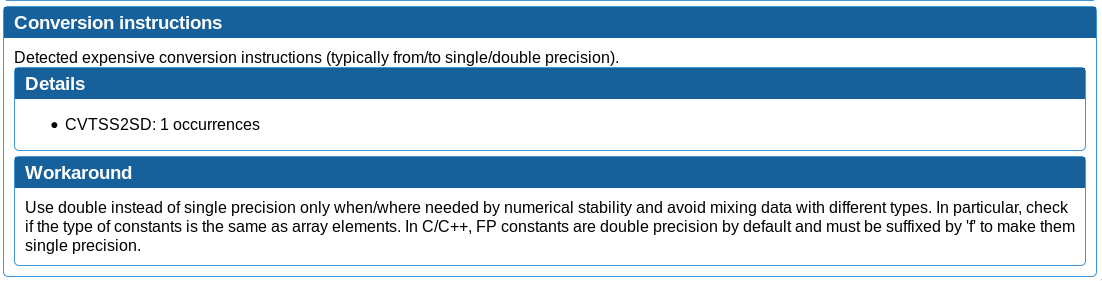
\includegraphics[scale=0.4]{./figures/L1/maqao_noopt_complex_instr.png}
    \caption{Rapport de MAQAO sur NOOPT : instruction complexe détectée.}
    \label{fig.maqao_noopt_complex_instr}
\end{figure}

\paragraph{Toutes les optimisations (OPT-BEST-L1)} Toutes les optimisations
(sauf la conversion de type et la parallélisation, n'apportant aucun gain) ont
été réunies dans un seul code. Aucune modification supplémentaire n'as été
apporté par rapport aux optimisations décrites au-dessus. On observe au final
un gain non-négligeable par rapport à la version originale (speed-up de 2.9).

\paragraph{Toutes les optimisations avec flags (OPT-BEST-L1-2)} Ce benchmark
correspond à la version du code étant la mieux optimisée, mais mesurée avec les
options de compilation donnant le meilleur résultat dans la phase 1. On observe
qu'on retrouve un léger gain par rapport à cette version du code sans ces
options de compilation (paragraphe précédent), mais qu'elle est moins rapide que
la version générée dans la phase 1, sans modification du code : en effet, on
obtient 7.5 cycles par itération sur cette version modifiée, contrairement à 4.5
cycles par itération sur la version originale. On en conclue que sur ce code, le
compilateur aura fait mieux que nous. La différence de performance s'explique
par le fait que nous n'avons pas tiré partit de la vectorisation, et que nous
forçons le compilateur à utiliser notre approximation de l'exponentielle. En
revanche, en lui laissant le libre arbitre, il a pu utiliser (dans la version
originale du code) une version vectorisée de l'exponentielle, ce qui fait toute
la différence ! Cette différence n'est pas visible dans le code assembleur pour
la fonction exponentielle car c'est un appel de fonction, elle n'a pas été
inlineé (\textit{call exp\_finite}). Cependant, MAQAO détecte très bien la
différence de vectorisation, comme illustré sur la
Figure~\ref{fig.maqao_noopt_vec} qui nous montre le degré de vectorisation du
code originale avec les bonnes options de compilation et la
Figure~\ref{fig.maqao_bestl1_vec} qui nous montre le degré de vectorisation du
code optimisé. En effet, on voit que dans notre code, nous pourrions obtenir un
gain considérable en vectorisant notre fonction exponentielle et notre boucle :
ici se trouve le goulet d'étranglement de notre programme.

\begin{figure}[p]
    \centering
    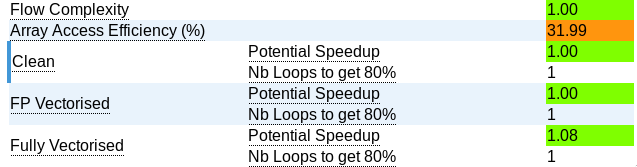
\includegraphics[scale=0.6]{figures/L1/maqao_noopt_flags.png}
    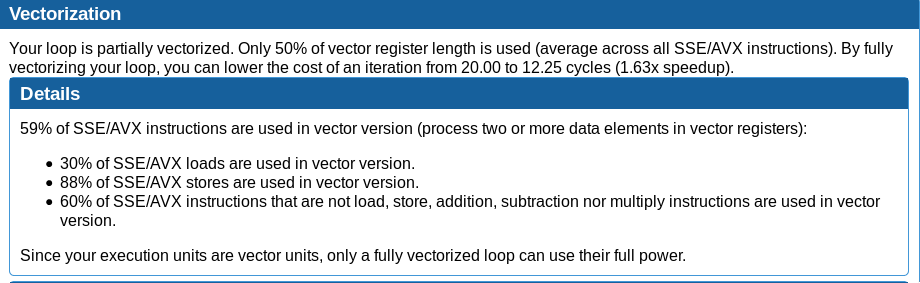
\includegraphics[scale=0.45]{figures/L1/maqao_noopt_flags_vec.png}
    \caption{Rapport de MAQAO sur NOOPT : vectorisation avec les bons flags}
    \label{fig.maqao_noopt_vec}
\end{figure}

\begin{figure}[h]
    \centering
    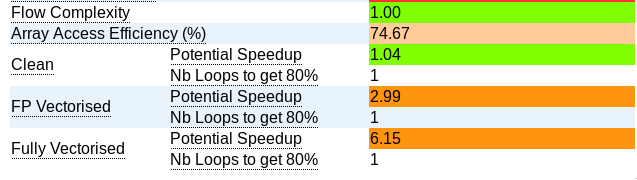
\includegraphics[scale=0.6]{figures/L1/maqao_bestl1_wflags.png}
    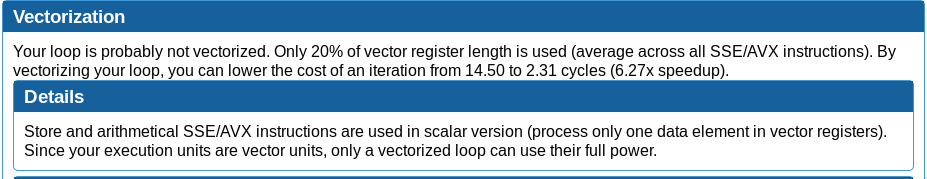
\includegraphics[scale=0.45]{figures/L1/maqao_bestl1_wflags_vec.png}
    \caption{Rapport de MAQAO sur BEST-L1 : vectorisation}
    \label{fig.maqao_bestl1_vec}
\end{figure}

\paragraph{Vectorisation} Comme identifier dans les paragraphes précédents, pour
obtenir un gros speed-up, il nous fallait vectoriser notre code. Nous avons
alors commencer à tenter une vectorisation en utilisant des \textit{intrinsics}.
Nous avons aussi analysé la version d'exponentielle vectorisée d'Agner Fog dans
son manuel d'optimisation. Cependant, nous n'avons pas réussis à venir à terme
de notre code : entre les \textit{intrinsics} de GCC et d'ICC, entre les
différents jeux d'instructions SIMD (SEE/2/3/4/4, AVX/512), entre les codes
pour le C et ceux pour le C++, et enfin entre les versions customs de fonction
vectorisée ou l'utilisation de bibliothèques mathématiques vectorisées (VML, IPP,
Sleef, SVML, VCL...), nous nous sommes un peu perdus. Je pense que nous aurions
dû commencer par vectoriser un code plus simple pour nous entraîner, peut-être
directement en assembleur pour avoir une compréhension maximale. Quoi qu'il en
soit, à cette heure, nous n'avons plus le temps de retenter l'expérience : mais
nous savons comment nous lancer et quel chemin suivre pour obtenir un speed-up
maximal.

\subsubsection{Cache L2}

\subsubsection{RAM}

\newpage
\section{Conclusion}

Pour conclure, nous aurons tout de même réussis à apporter des optimisations que
nous jugeons intéressantes à notre kernel. Au départ, le temps de calcul d'une
itération de notre boucle (une fonction exponentielle, une multiplication et une
conversion de type float vers double) était d'environ 23s. Après nos
optimisations manuelles, une itération du kernel prenait environ 8s, soit
presque 3 fois plus rapide ! Malheureusement, nous ne sommes pas parvenus à
atteindre la rapidité de calcul obtenue par les meilleures options du
compilateur, à savoir 4,5s. Nous pensons qu'avec la vectorisation de notre
fonction exponentielle et de notre boucle intérieur du kernel, cela aurait pu
être possible de faire mieux !
Nous aurons été confrontés à de nombreux petits soucis épars pendant notre
démarche, classique pour des étudiants découvrant les outils de mesures de
performances, résultants parfois à des problèmes de cohérences entre les
mesures. Ces problèmes de cohérences pouvaient avoir des explications diverses :
utilisation du CPU par un autre processus, erreurs dans le code, mauvais
paramétrage de l'outil de mesure... D'où l'importance de la rigueur de mesure
apprise en TD, détaillée dans le rapport.

Pour conclure, nous pensons que ce projet nous aura apporté une bonne méthode
d'analyse et d'optimisation, et nous aura permis de mettre en application réelle
les techniques et sujets vus en cours. Une très bonne première approche !

\end{document}
